% Generated by scripts/md_to_pmlr.py from nesy_body.md + nesy_supplementary.md.
% Do not edit by hand: change the markdown (which verify_draft.py checks) and regenerate.
\documentclass[anon]{nesy2026} % anonymised submission for OpenReview

\usepackage{booktabs}
\usepackage{tabularx}

\title[Knowledge the Network Already Has]{Knowledge the Network Already Has: An Exogeneity Precondition for Neuro-Symbolic Intrusion Detection}
% Author block is suppressed by the anon option; fill in only for the camera-ready.
\clearauthor{\Name{Author Name} \Email{author@example.org}\\ \addr Address}

\begin{document}
\maketitle

\begin{abstract}
When does injecting symbolic knowledge into a neural model help? For intrusion detection we give a precise answer, a mechanism for it, and a benchmark on which the question cannot be tested. \textbf{The neuro-symbolic intrusion detectors that report gains share an unstated property: the knowledge they inject is information the network cannot compute from its input} --- an asset inventory, a relational graph, an external attack taxonomy. Our own symbolic pillar did the opposite. Its Logic Tensor Network axioms are deterministic functions of the flow features the network already reads, and it was null alone ($-$0.0004, n.s.) and significantly harmful when stacked (0.6926 $\rightarrow$ 0.6708, p $<$ 0.0001). We propose that \textbf{symbolic knowledge helps exactly to the extent it lies outside the model's learned feature basis}, and show that the same property explains a second failure: a closed-set learner reaches a novel attack family only insofar as its signature overlaps that basis. For Bot the overlap is empty (\textbf{0 of 8} discriminative features shared), every flow is classified benign, and the model's ranking of it is noise (cross-seed $\rho$ = \textbf{$-$0.090}). This survives five attempts to break it, including a capture where Bot is abundant and corrected labels. We then try to satisfy the precondition on CIC-IDS2017 and cannot: host-role knowledge built from metadata the network never sees is still predicted from its features at AUC \textbf{0.990--0.994}. \textbf{Exogenous knowledge cannot be manufactured by aggregating the same data}, so a benchmark with no external knowledge artefact cannot support the experiment its neuro-symbolic results depend on.
\end{abstract}

\section{Introduction}\label{sec:1}

Neuro-symbolic learning promises that domain knowledge, stated as logic, can supply what data alone does not. Intrusion detection is an attractive test: attacks absent from training are exactly where a data-driven detector is weakest, and exactly where knowledge of how networks and attacks behave ought to help.

We built a neuro-symbolic intrusion detector to test that promise, and it failed. Its Logic Tensor Network axioms --- over behaviours such as burst traffic, packet-size variance and beacon-like periodicity --- contributed \textbf{$-$0.0004} macro zero-day PR-AUC alone (not significant) and \textbf{harmed} the system significantly when stacked on a knowledge-graph channel (0.6926 $\rightarrow$ 0.6708, p $<$ 0.0001). This paper is about why, and the answer turns out to be general.

\textbf{The published systems that report gains share a property ours lacked.} \citet{grov2024} add a single axiom --- \emph{flows not communicating with web servers cannot be web attacks} --- and roughly double web-attack precision. KnowGraph \citep{zhou2024} reasons over relational structure between entities and lifts true positives from \textbf{0.0 \% to 35.5 \%} at a 0.5 \% false-positive rate, where the neural baseline detects nothing. \citet{kalutharage2025} align alerts to an external attack taxonomy. In each case \textbf{the knowledge is information the network cannot compute from its own input}. Every one of our behaviour predicates, by contrast, is a deterministic function of the flow features the network already reads. Ours supplied an inductive bias; theirs supplied evidence.

We state this as a precondition --- \textbf{symbolic knowledge helps a neural detector to the extent it lies outside the model's learned feature basis} --- and make three contributions around it.

\begin{enumerate}
  \item \textbf{One principle, two consequences (Sections~\ref{sec:3}--\ref{sec:4}).} The same property governs \emph{novel attack families}: a closed-set learner reaches a family it never saw only insofar as that family's signature overlaps the features it learned. Symbolic knowledge inside the basis adds nothing; a novel class outside it cannot be reached.
  \item \textbf{A durability test (Section~\ref{sec:5}).} The unreachability survives five attempts to break it: a capture where the family is abundant rather than rare, corrected labels, an explicitly trained reject class, cross-dataset augmentation, and a broad architecture and out-of-distribution sweep.
  \item \textbf{A negative evaluability result (Section~\ref{sec:6}).} Built from metadata the network never sees, host-role knowledge is still recovered from its features. A benchmark with no external knowledge artefact cannot support the experiment published neuro-symbolic gains rest on.
\end{enumerate}

\begin{figure}[htbp]
\floatconts
  {fig:thesis}
  {\caption{\emph{One principle, two consequences.} Both panels draw the same learned feature basis --- the features a closed-set objective selects. \textbf{(a)} Symbolic knowledge can help only from outside that basis: our Logic Tensor Network axioms are functions of the flow features and add no evidence, whereas the knowledge behind published gains \citep{grov2024,zhou2024,kalutharage2025} is not computable from the input. \textbf{(b)} An unseen attack family is reachable only insofar as it overlaps the basis: Web Brute Force shares 1 of 8 discriminative features and is reached only weakly once label artefacts are removed (Section~\ref{sec:7}); Bot shares none and is unreachable. Inside and outside map to opposite outcomes in the two panels.}}
  {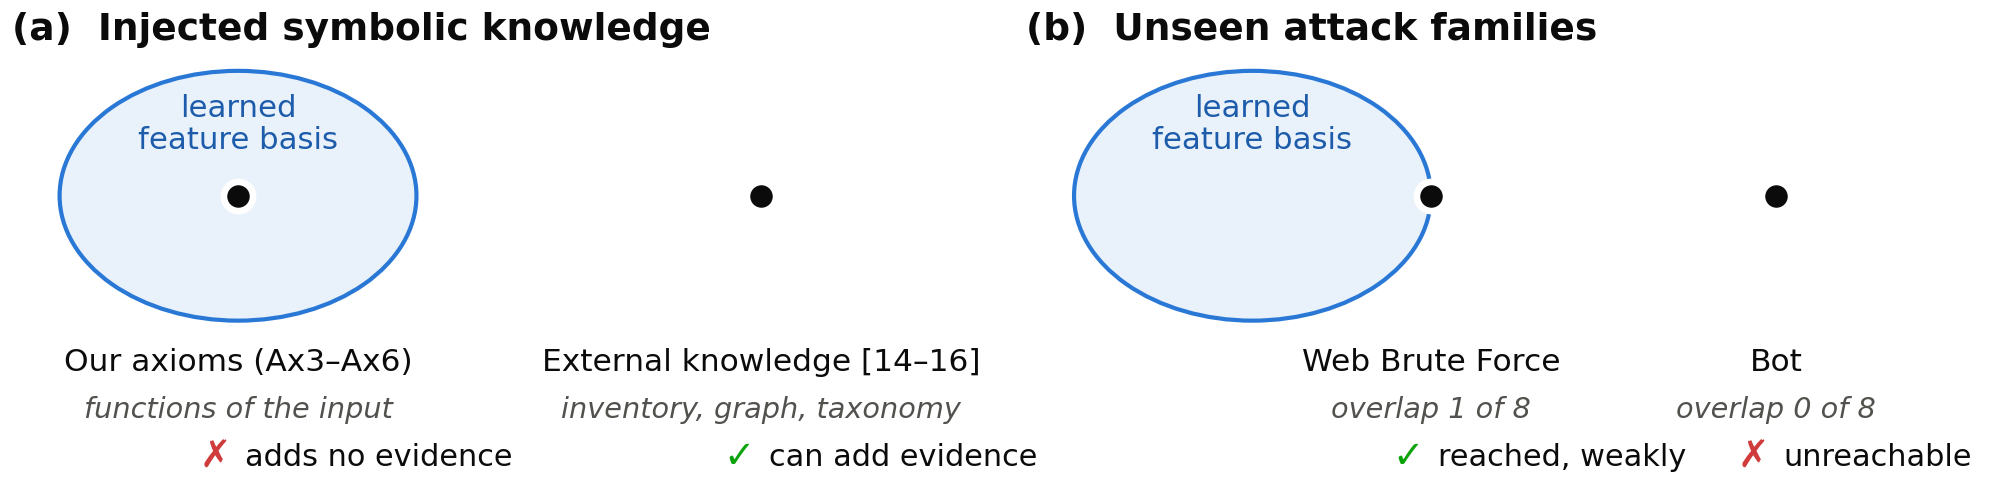
\includegraphics[width=\linewidth]{figures/nesy_fig1_thesis}}
\end{figure}

\textbf{Two measurement failures bound the magnitudes (Section~\ref{sec:7}), and we demonstrate both on our own system.} The metric the field reports cannot resolve zero-day capability, and on corrected labels two of our three headline zero-day families were measuring whether the dataset counts an unsuccessful connection attempt as an attack. They limit what we can claim quantitatively; they do not move the mechanism.

\section{Setting and measurement}\label{sec:2}

\textbf{Data.} CIC-IDS2017 \citep{sharafaldin2018} flow features, \textbf{68 numeric features per flow}. Nine attack families plus benign are \emph{known} and split 80/10/10 stratified, benign under-sampled to 1:1: \textbf{883,796 train / 110,475 validation / 114,658 test}. Six rare families --- Bot, Heartbleed, Infiltration, and Web Attack Brute Force / XSS / SQL Injection --- appear \textbf{only in test}.

\textbf{Metric.} Macro zero-day PR-AUC over the three adequately powered unseen families: \textbf{Bot (n = 1,956), Web Attack Brute Force (n = 1,507), Web Attack XSS (n = 652)}. Heartbleed (n = 11), Infiltration (n = 36) and SQL Injection (n = 21) are excluded as underpowered. Where test sets differ in prevalence --- across datasets or labellings --- we compare only \textbf{lift} (PR-AUC $\div$ prevalence), since PR-AUC is bounded below by prevalence; chance lift is 1.0.

\textbf{Reproducibility floor.} Training is not bit-reproducible at a fixed seed without determinism flags, so we measured the floor before interpreting any delta: nondeterminism SD \textbf{0.0222}, seed SD \textbf{0.0171} (determinism on, n = 6), data-split SD \textbf{0.0228}, giving \textbf{0.0285} of uncertainty on an absolute number. \textbf{Every comparison is paired on seed}, and a delta is reported as established only when its direction is consistent across seeds; magnitudes are given as ranges. This floor retracted one of our own headline claims, a gap of 0.9 SD that a paired bootstrap had called significant at p = 0.001 (Appendix~\ref{apd:E}).

\section{A symbolic pillar that could not help}\label{sec:3}

\textbf{The architecture.} A 1D CNN over the flow features, a Logic Tensor Network \citep{badreddine2022} layer grounding fuzzy axioms in network behaviours, and a knowledge-graph channel scoring cluster growth over time. The axioms (Ax3--Ax6) constrain the network's attack output by behaviour predicates --- large packets with high packet-size variance, burst traffic, scan-like probing, beacon-like periodicity.

\textbf{The result.} Across every injection point we tried --- loss-level, representation-level and inference-level --- the symbolic pillar costs macro zero-day PR-AUC or changes nothing. Alone it contributes \textbf{$-$0.0004 (n.s.)}; stacked on the knowledge graph it \textbf{significantly harms} the system (0.6926 $\rightarrow$ 0.6708, \textbf{p $<$ 0.0001}), diluting Bot from 0.2518 to 0.2043. An axiom that briefly appeared to help Bot did not survive multi-seeding. This is not a tuning failure: it is consistent in sign across every configuration.

\textbf{What the successful systems share.} The contrast with published gains is the diagnostic:

\begin{center}\small
\begin{tabularx}{\linewidth}{l>{\raggedright\arraybackslash}X>{\raggedright\arraybackslash}X}
\toprule
\textbf{system} & \textbf{knowledge injected} & \textbf{computable from the flow features?} \\
\midrule
\citet{grov2024} & \emph{non-web-server flows cannot be web attacks} & \textbf{no} --- requires an asset inventory \\
KnowGraph \citep{zhou2024} & logic over entity-relational structure & \textbf{no} --- requires a relational graph \\
\citet{kalutharage2025} & technique mapping to an attack taxonomy & \textbf{no} --- requires an external taxonomy \\
\textbf{ours} & behaviour predicates (Ax3--Ax6) & \textbf{yes} --- each is a function of the input \\
\bottomrule
\end{tabularx}
\end{center}

All seven of our behaviour predicates are deterministic functions of features the network consumes: \texttt{HighEntropy} is packet-length standard deviation, not Shannon entropy; \texttt{BeaconLike} is a function of destination port. A predicate the network can already compute cannot tell it anything; it can only reshape the hypothesis space, which is regularisation. \textbf{The injected knowledge was endogenous.}

\textbf{The precondition.} We therefore propose: \emph{symbolic knowledge helps a neural detector to the extent that it lies outside the model's learned feature basis.} The next section shows the same property governs a second, apparently unrelated failure.

\section{One principle, two consequences}\label{sec:4}

A closed-set discriminative model learns only the features that separate the classes in its training objective. It follows that a class it never saw is reachable \textbf{exactly to the extent its signature overlaps that learned basis} --- the same statement as Section~\ref{sec:3}'s precondition, with a novel class in place of an injected predicate. Where the overlap is empty, the model's output on that class is not merely poor but \textbf{unstable}, because nothing in the objective constrains it.

We establish this on Bot, where the overlap is empty:

\begin{itemize}
  \item \textbf{100 \% of Bot flows are classified BENIGN}, mean p(BENIGN) = \textbf{0.9984}, on all three seeds. Bot is not ambiguous to the model; it is confidently asserted benign, which defeats every confidence-based remedy before it is tried.
  \item The eight features separating Bot from benign share \textbf{0 of 8} with the eight the known-class task selects.
  \item The model's Bot ranking is therefore \textbf{noise} (Figure~\ref{fig:mechanism}): cross-seed Spearman \textbf{$\rho$ = $-$0.090}, against 0.68--0.83 for every other family. RandomForest behaves identically ($\rho$ = 0.068); \textbf{the autoencoder does not ($\rho$ = 0.827)}, so the property belongs to closed-set discriminative learning rather than to neural networks. Three seeds cannot distinguish $-$0.090 from $-$0.02; they are ample to show it is not 0.7, and only that is load-bearing.
  \item \textbf{The information is present.} An oracle given Bot labels reaches PR-AUC \textbf{0.9988} from the same features. The oracle trains on zero-day labels and is an upper bound, not a method; it shows the barrier is supervision, not information or modality.
\end{itemize}

\begin{figure}[htbp]
\floatconts
  {fig:mechanism}
  {\caption{\emph{Bot's ranking is noise for closed-set learners.} Agreement between each model's rankings of test flows across three training seeds (Spearman $\rho$), per unseen family. For Bot the two closed-set discriminative learners do not agree with themselves (1D CNN $-$0.090, random forest +0.068); the benign-only autoencoder does (+0.827), so the instability belongs to closed-set discriminative learning rather than to neural networks. The zero line marks no agreement; no threshold is drawn, because none is measured. Three seeds cannot distinguish $-$0.090 from $-$0.02, but they suffice to show it is not 0.7.}}
  {
\includegraphics[width=\linewidth]{figures/nesy_fig2_mechanism}}
\end{figure}

\textbf{The two consequences side by side.} Knowledge \emph{inside} the basis --- our axioms --- adds no evidence. A novel class \emph{outside} the basis --- Bot --- cannot be reached. Both follow from what a closed-set objective does and does not constrain. \textbf{The reachable direction is weaker than the unreachable one} (Section~\ref{sec:7}): the evidence that overlapping families \emph{are} reached rested on web-attack scores that corrected labels largely remove. The \textbf{ordering} survives; the magnitudes do not.

\section{Durability: five attempts to break it}\label{sec:5}

A mechanism asserted once is a hypothesis. We pre-registered a falsifier for each of the following before running it.

\begin{center}\small
\begin{tabularx}{\linewidth}{>{\raggedright\arraybackslash}X>{\raggedright\arraybackslash}X>{\raggedright\arraybackslash}X}
\toprule
\textbf{attempt} & \textbf{what it controls for} & \textbf{result for Bot} \\
\midrule
\textbf{Independent capture}, CSE-CIC-IDS2018, training size matched & that Bot is merely \emph{rare} & Bot is \textbf{abundant} and scores \textbf{0.83$\times$} chance --- below a random ranker \\
\textbf{Corrected labels} \citep{engelen2021}, attack flows with no payload excluded & a labelling artefact & effective Bot (n = 738) lifts \textbf{0.57 / 0.64 / 8.99} --- two of three seeds below chance \\
\textbf{Explicit reject class}, three known families merged into \texttt{UNKNOWN} & that the model was never \emph{asked} to reject & ceiling is chance: \textbf{+0.068} with the sign flipping between seeds \\
\textbf{Cross-dataset augmentation}, 2018's known pool added & that the basis was too narrow & \textbf{$-$0.1461} macro against a seed-matched control, 0/3 seeds better \\
\textbf{Sweep}: 4 deep architectures, 7 classical, 4 benign-only, 9 OOD scorers & method choice & none reaches Bot; the best OOD scorer reaches 0.0783 against a pre-set 0.08 threshold \\
\bottomrule
\end{tabularx}
\end{center}

\textbf{The corrected-label result is the most demanding, and how it fails to falsify matters.} The criterion was lift above chance \emph{consistently across seeds}. A mean of 3.4$\times$ would read as detection; it describes no run that happened. The spread is itself Section~\ref{sec:4}'s instability signature.

\textbf{The reject class yields the most informative positive.} Two merges differing only in \emph{what} was merged into \texttt{UNKNOWN} produce a \textbf{double dissociation}, direction-consistent on every seed for every family: a homogeneous merge of three DoS variants anti-ranks Bot ($-$0.206) while reaching the web families best, and a heterogeneous merge reverses both (Bot contrast \textbf{+0.274, 2.57$\sigma$, 3/3}). A reject class is therefore not a generic "none of the above": \textbf{its reach is set by the feature basis of what is merged into it} --- Section~\ref{sec:4}'s mechanism observed in the open-set case, with chance as its ceiling for Bot.

\textbf{Augmentation fails for a reason that is itself instructive.} Adding a related attack family from another capture sharpened one decision region until it mis-fired on the original capture's benign traffic: benign flows outscoring the Web Brute Force median rose from \textbf{2 to 242}, 81 \% of them assigned to \texttt{SSH-Patator}. A wider basis in directions already covered imports false positives rather than reach.

\section{Evaluability: the benchmark cannot supply exogenous knowledge}\label{sec:6}

If Section~\ref{sec:3}'s precondition is right, the constructive move is to inject knowledge from outside the basis. We attempted this on CIC-IDS2017 and the attempt failed at the premise --- which is the result.

\textbf{Construction.} Source and destination IP addresses are \emph{not} among the features, and no single flow's vector expresses a property of a host across many flows. We therefore built host-role predicates from flow metadata: whether a destination normally serves a port, whether a flow's port is unusual for its host, a source's fan-out, and pair persistence. Profiles are built from \textbf{training flows only}, so the construction is inductive rather than transductive. Attacker identity is \textbf{deliberately excluded}: the testbed documents the attacker subnet, and conditioning on it would be label leakage dressed as domain knowledge.

\textbf{The premise test.} A predicate is exogenous only if the network could not already compute it. We fitted gradient-boosted models to predict each predicate \emph{from the flow features}:

\begin{center}\small
\begin{tabular}{lrr}
\toprule
\textbf{predicate} & \textbf{all features} & \textbf{without \texttt{Destination Port}} \\
\midrule
Unusual port for host & AUC 0.990 & 0.988 \\
Host serves a web port & AUC 0.994 & 0.992 \\
Source fan-out & R$^{2}$ 0.949 & 0.898 \\
Pair persistence & R$^{2}$ 0.914 & 0.886 \\
\bottomrule
\end{tabular}
\end{center}

\textbf{None is exogenous.} The ablation is what makes this a finding rather than an artefact: dropping the one port feature barely moves the numbers, so the flow's own port is not giving the answer away --- the remaining features determine host role and cross-flow structure by themselves. In a testbed where each host plays one scripted role, a flow's characteristics nearly identify its host, and therefore that host's aggregate properties.

\textbf{The generalisable claim.} \emph{Exogenous knowledge cannot be manufactured by aggregating the same data.} Grov et al.'s axiom works because an asset inventory is an artefact from \textbf{outside} the capture; ours was inferred \textbf{from} it, and anything inferable from the capture is largely inferable from its features. CIC-IDS2017 ships no inventory, topology or threat intelligence, so \textbf{the neuro-symbolic approach as the literature practises it cannot be evaluated on this benchmark.} We did not run the injection arms: measuring a predicate the model can already compute would report feature engineering as a symbolic result. The thresholds (AUC $<$ 0.75, R$^{2}$ $<$ 0.5) are conventions, and a predicate at R$^{2}$ = 0.90 leaves residual variance; a stronger predictor would only strengthen the conclusion.

\section{What limits the magnitudes}\label{sec:7}

Two measurement failures bound how far any number here should be trusted. We report both because the second one retracts two of our own headline families.

\textbf{Label semantics.} \citet{engelen2021} re-ran CIC-IDS2017 through a corrected flow meter and introduced an \texttt{X -- Attempted} label for attack flows that transmitted \textbf{no payload}. Two-thirds of Bot and roughly nine-tenths of the web families are such flows. Retraining on the corrected release:

\begin{center}\small
\begin{tabular}{lrrr}
\toprule
\textbf{family} & \textbf{attempted folded in} & \textbf{attempted excluded} & \textbf{n (excluded)} \\
\midrule
Web Attack Brute Force & \textbf{29.4$\times$} & \textbf{2.1$\times$} & 151 \\
Web Attack XSS & 61.5$\times$ & \emph{unmeasurable} & 27 \\
\bottomrule
\end{tabular}
\end{center}

\textbf{Web Brute Force falls from PR-AUC 0.8861 to 0.0072} once flows that transmitted nothing are removed. Its apparent reachability was substantially detection of bare connection attempts, which are trivially unlike normal traffic. \textbf{A better metric on a mislabelled benchmark is still the wrong measurement.} This is why Section~\ref{sec:4}'s reachable direction is weak; it does not touch the unreachable one, which Section~\ref{sec:5} tested on exactly these labels.

\textbf{Metric resolution.} The metric the field publishes cannot resolve the capability it is used to claim. Across 31 methods evaluated identically, \textbf{37 of 169 method pairs (22 \%)} are statistically indistinguishable on it while differing by a factor of two or more in macro zero-day PR-AUC; the worst pair is \textbf{0.0052} apart on the former and \textbf{16.6$\times$} apart on the latter. The metric is neither noisy nor uninformative ($\rho$ = +0.582 against zero-day performance) --- it is too coarse where the field reports. Full analysis in Appendix~\ref{apd:B}.

\textbf{The one component that helps.} A knowledge-graph channel scoring cluster growth over time improves macro zero-day PR-AUC; its cluster count was selected on test, so the honest improvement is the held-out one, \textbf{+0.0305 at 2.86$\sigma$} on a half never used for selection. Its signal rides substantially on CIC-IDS2017's scripted attack windows, and temporal burstiness of a raw-feature cluster does not require a knowledge graph; we do not claim it as evidence for the neuro-symbolic approach (Appendix~\ref{apd:D}).

\section{Related work}\label{sec:8}

\textbf{Neuro-symbolic intrusion detection.} Logic Tensor Networks \citep{badreddine2022} supply the fuzzy-logic-to-loss machinery. \citet{bizzarri2024} apply it to CIC-IDS2017 with a hybrid cross-entropy and satisfiability loss and report improved unknown-attack accuracy; that paper is our starting point, and a survey by the same group \citep{bizzarri2025survey} places it in a growing literature. \textbf{We reproduce its CNN and cannot reproduce its symbolic gain}: on its own metric we obtain 47.85 \% against its 48.34 \% for the CNN, while our nearest reproduction of the hybrid scores 47.24 \%. The comparison is in form rather than head-to-head --- the modality and zero-day membership differ. The gains in \citep{grov2024,zhou2024,kalutharage2025} are, by our reading, gains from \textbf{exogenous} knowledge; we make that property explicit, test it, and show a widely used benchmark cannot satisfy it. This is not a criticism of those works, whose knowledge genuinely is exogenous: the point is that the property is load-bearing and usually left implicit, so a reader cannot distinguish a knowledge result from a feature-engineering result without it. A survey \citep{hakim2025} notes that most neuro-symbolic cybersecurity evaluations are limited by evaluation gaps.

\textbf{The benchmark.} CIC-IDS2017 \citep{sharafaldin2018} is widely reported on. \citet{engelen2021} documented defects in flow construction and labelling and released corrected processing; a follow-up quantified the effect on detection \citep{lanvin2023}, and a survey of 89 intrusion datasets argues data quality now limits the field \citep{goldschmidt2025}. We add a consequence for the zero-day question specifically, and a second property the benchmark lacks: any external knowledge artefact.

\textbf{Closed worlds and security machine learning.} \citet{sommer2010} argued that intrusion detection is hostile to machine learning because the interesting events lie outside the closed world. Section~\ref{sec:4} supplies a mechanism for one instance and shows the failure is instability, not only inaccuracy. \citet{arp2022} catalogue ten pitfalls in security machine learning; we audit this work against all ten in Appendix~\ref{apd:E}, and two --- lab-only evaluation and threat model --- we do not address.

\textbf{Open-set recognition and OOD scoring.} Treating unseen attacks as an open-set problem has a long history \citep{cruz2017}; post-hoc scorers need no retraining \citep{hendrycks2017,liang2018,liu2020}. None rescues Bot (Section~\ref{sec:5}).

\section{Limitations and conclusion}\label{sec:9}

\textbf{Limitations.} Two captures from the same producer under related methodology are not evidence of generality across network environments. Only two zero-day families are adequately powered under corrected labels. Flow features, not payload bytes, are used throughout, though the oracle shows the barrier is not modality. Our exogeneity thresholds are conventions. We do not evaluate adversarially, and nothing is deployed.

\textbf{Conclusion.} Symbolic knowledge helps a neural intrusion detector to the extent that it lies outside the model's learned feature basis. The same property makes a novel attack family with no overlap unreachable, and that unreachability survived every attempt we made to break it. The neuro-symbolic systems that report gains inject genuinely exogenous knowledge; ours did not, and on CIC-IDS2017 we could not construct any, because knowledge aggregated from a capture is recoverable from that capture's features. \textbf{Before reporting a neuro-symbolic gain, establish that the knowledge injected is not already in the input --- and recognise that a benchmark may make that impossible.}

\emph{Code, per-run records and trained models will be released upon acceptance.}

\bibliography{refs}

\appendix

\section{Protocol and metric, in full}\label{apd:A}

\subsection{Protocol and metric}

\textbf{Data and split.} CIC-IDS2017 flow features, \textbf{68 numeric features per flow}. Nine attack families plus benign are treated as \emph{known} and split 80/10/10 stratified, with benign under-sampled to 1:1: \textbf{883,796 train / 110,475 validation / 114,658 test}. Six rare families --- Bot, Heartbleed, Infiltration, and Web Attack Brute Force / XSS / SQL Injection --- appear \textbf{only in test} and are never trained on. Note that PortScan and DDoS are \emph{known, trained-on} classes under this protocol; claims resting on their detection do not transfer to the zero-day setting.

\textbf{Headline metric.} \textbf{Macro zero-day PR-AUC}, averaged over the three adequately powered unseen families: \textbf{Bot (n = 1,956), Web Attack Brute Force (n = 1,507), Web Attack XSS (n = 652)}. Heartbleed (n = 11), Infiltration (n = 36) and SQL Injection (n = 21) are \textbf{excluded as underpowered} and are never reported to four decimal places.

We do not headline the blended "benign versus all unknowns" figure. It is a \textbf{size-weighted mixture that reorders the ranking}, and we know this because it produced a claim of ours --- "XGBoost $\approx$ CNN" --- that we retracted on the strength of the mixture and later had to \emph{un}-retract when a paired test showed the original claim was right (p = 0.80, n.s.). We cite that episode as evidence for the metric choice, and it is our own error.

\textbf{Duplicate rows, and why the asymmetry is the finding.} 17.0 \% of test rows are exact feature-vector duplicates of training rows. De-duplicating costs the supervised channels 0.0035--0.0049 on the published metric. It costs the zero-day metric \textbf{nothing}, because all six zero-day families measure \textbf{0.0 \% overlap} with training. Duplication therefore inflates \emph{the field's} metric and leaves \emph{ours} untouched --- this is a property of the comparison, not a flaw in our numbers.

\textbf{Feature transform.} We use \texttt{log1p}, justified \textbf{on the headline metric}: 0.6299 $\pm$ 0.0031 against 0.1606 $\pm$ 0.0039 for raw features, over three seeds per arm (Welch t = 163). We note plainly that our \emph{original} justification for this choice cited the contaminated overall-binary metric, and that the A/B was re-run on the correct metric. The conclusion was right and its justification was wrong; those are separate facts, and the re-run was necessary regardless of which way it came out.

\section{The metric-resolution gap, in full}\label{apd:B}

\subsection{The metric failure}

The CIC-IDS2017 literature reports accuracy, F1 and AUC above 99 \% with enough regularity that the numbers have stopped discriminating. That would be unremarkable if those numbers were used only to claim what they measure --- separating benign traffic from attack families the model was trained on. They are not. They are routinely offered as evidence of capability against \emph{novel} attacks, which is the capability that matters operationally and the one the metric is least able to speak to.

We make that gap quantitative. \textbf{The 40 methods are ours, and that matters for how the claim should be read.} They are not 40 published systems re-run; they are 40 models we trained under one protocol --- classical baselines, deep architectures, benign-only anomaly detectors, neuro-symbolic variants and fusions --- precisely so that every one is scored identically on both axes, which published numbers never are. \textbf{The step from "these 40" to "the literature" is therefore an argument, not a measurement}, and it rests on two things we can check: the 40 span the algorithm families the field publishes, and \textbf{they land inside the field's own reported band} (0.977--0.993 on the published metric). Scoring each on that metric and on \textbf{macro zero-day PR-AUC} over held-out families, we find:

\begin{itemize}
  \item \textbf{37 of 169 comparable method pairs (22 \%) are indistinguishable on the published metric while differing $\geq$2$\times$ on zero-day capability.} "Indistinguishable" means a difference below \textbf{0.0060}, two standard deviations of a \emph{difference} derived from a measured median run-to-run SD of \textbf{0.0021}. We state the band rather than the count alone, because the count is meaningless without it.
  \item The extreme case, \texttt{deep\_cnn\_lstm} versus \texttt{linear\_svm}, sits \textbf{0.0052 apart on the published metric and 16.6$\times$ apart on zero-day}. We give the extreme only alongside the distribution above; on its own it would be cherry-picking.
  \item Restricting to the field's own reporting regime --- the 22 methods scoring $\geq$0.98, which is where published work lives --- those methods sit \textbf{within 0.0144 of one another and span 18.5$\times$} on zero-day. The $\geq$0.98 cut is chosen \emph{because it is the field's regime}, not because it separates the data.
\end{itemize}

\textbf{These figures exclude 11 tie-degenerate scorers, and the exclusion is not optional.} Of the 42 methods we evaluated, eleven --- \texttt{decision\_tree}, \texttt{knn\_k5}, \texttt{naive\_bayes}, four LTN variants and the four knowledge-graph channels --- place roughly half of all flows in a \textbf{single tie block}. this appendix explains why that makes their PR-AUC incomparable to a continuous scorer's, and a "$\geq$2$\times$ apart on macro" test is precisely a comparison of PR-AUCs. Including them gives \textbf{75 of 249 pairs (30 \%)} and a headline extreme of 17.9$\times$; both are inflated by the same artefact the paper elsewhere warns about, so we report the excluded population and give the inclusive figures here rather than quietly choosing the larger one. \textbf{The claim survives the exclusion --- 22 \% and 16.6$\times$ --- and the rank correlation barely moves (+0.589 $\rightarrow$ +0.582).}

\textbf{Two stronger versions of this claim are false and we do not make them.} The published metric is not uninformative about zero-day performance: Spearman $\rho$ = \textbf{+0.582} (p = 0.0006) over the non-degenerate methods, \textbf{+0.589} over all 42, and it stays positive within the $\geq$0.98 regime. Nor is its spread within its own noise: it is a \emph{precise} measurement, with a median run-to-run SD of 0.0021, roughly ten times below its spread across methods. The metric is precise, weakly informative, and \textbf{too coarse in the regime that matters} --- which is a narrower and more useful statement than either strong form, and it is the one our data support. Both refutations are hard-coded into the output of the script that produces the figure, so the strong forms cannot be reintroduced by accident.

\textbf{Contributions.}

\begin{enumerate}
  \item A resolution failure, demonstrated across 42 methods scored on a single axis (this appendix, Fig. 1).
  \item A mechanism for why zero-day detection is hard rather than merely unmeasured, with four independent symptoms traced to one cause (Appendix~\ref{apd:C}).
  \item A negative result that is expensive to obtain: four categories of method, a standard OOD battery, two post-hoc remedies and our own symbolic architecture all fail in the same way (Appendix~\ref{apd:D}).
  \item One partial success and its honest bound (Appendix~\ref{apd:D}), and a measurement-discipline section that retracts two of our own claims (Appendix~\ref{apd:E}).
\end{enumerate}

\subsection{The gap, demonstrated four independent ways}

\textbf{(a) One model, two protocols.} Holding the model fixed and changing only the evaluation protocol moves XGBoost from \textbf{0.9936 to 0.6372} and our CNN from \textbf{0.9928 to 0.6446} --- a gap of \textbf{0.3564} produced by nothing but the question asked.

\textbf{(b) Seven classical baselines.} All seven land in \textbf{0.977--0.985} on the published metric, against the CNN's 0.9928 --- the field's regime. On zero-day they span \textbf{0.0374 to 0.6049, a factor of 16}. Logistic regression is \textbf{98 \% as good as the CNN on the published metric and 17$\times$ worse on zero-day.} Two members of this tier are \textbf{score-degenerate}: \texttt{decision\_tree} and \texttt{knn} place 50.1 \% and 49.8 \% of all flows in a single tie block, so their PR-AUC is not comparable to a continuous scorer's. \textbf{This is the same property that removes eleven methods from the headline figures above} --- it is a general exclusion criterion in this paper, not a Tier-A footnote, and the analysis reports both populations so the effect of applying it is visible rather than assumed. The best \emph{valid} Tier-A result is the MLP at a three-seed mean of \textbf{0.4965} --- not the n = 1 figure of 0.5360 that a single run reported. \textbf{k-NN is not citable at all}: its macro spans 0.0440--0.4270 across seeds, because the only thing the seed changes is which 50,000 rows it memorises.

\textbf{(c) Four deep architectures.} Published metric \textbf{0.9854--0.9932}. The relationship with zero-day capability is not merely weak here, it is \textbf{inverted}: the tier's \emph{worst} zero-day model (Transformer, macro 0.1106) posts 0.9894, while \texttt{deep\_gru} (macro 0.3029) posts the tier's \textbf{highest} published score, 0.9932. Three caveats travel with this tier. The recurrent models run over the \textbf{feature axis, not time} --- the 68 statistics are unordered --- which matches published practice and is therefore the right comparison, but is \textbf{not evidence about sequence modelling}. Budgets are unmatched (the LSTM hit its 30-epoch cap). The Transformer result is \textbf{one under-tuned configuration}, not a claim about attention.

\textbf{(d) The base paper's own metric set.} Evaluated on Bizzarri et al.'s five views, we exceed their reported figures by 18--29 pp on all four known-class views and \textbf{reproduce their 1D CNN's zero-day accuracy almost exactly --- 47.85 \% against 48.34 \%.} What we cannot reproduce is their Hybrid-LTN's \textbf{+12 pp symbolic gain}: our closest reproduction of their model scores \textbf{47.24 \%}, no better than our own CNN. This is a comparison in \textbf{form, not head-to-head} --- different modality (flow features versus payload bytes), zero-day membership differing by a swap (they hold out PortScan and train Infiltration; we do the reverse), and different class sizes. Holding the model fixed and changing only the family mix moves their headline from 48.32 \% to 44.38 \%, so \textbf{composition explains roughly 4 pp of the missing 12} --- it is not explained away, but we say what is controlled.

\subsection{Two defects in that zero-day metric, verified arithmetically}

\textbf{It has no false-positive term.} Their zero-day view contains only attack rows, so precision $\equiv$ 1, accuracy \emph{is} recall, and F1 = 2A/(1+A) exactly --- we reproduce every published F1 from its matching accuracy to within 0.02 pp. The headline "accuracy 48 $\rightarrow$ 60 \%, F1 65 $\rightarrow$ 75 \%" is therefore \textbf{one result reported twice}, and \textbf{a model that flags every flow scores 100 \% on both}. We know this failure mode is reachable because a float32 saturation bug in our own pipeline did exactly that, and was caught only because our metric has a benign side. \textbf{It is also a size-weighted mixture}, the same defect described in Appendix~\ref{apd:A}.

\section{The mechanism, extended}\label{apd:C}

\subsection{The mechanism --- why a closed-set model cannot reach a novel class}

The gap in Appendix~\ref{apd:B} is not merely unmeasured; it is hard, and we can say why.

\textbf{The synthesis.} A closed-set discriminative model learns only those features that separate the classes present in its training objective. A novel class is therefore reachable exactly to the extent that its signature overlaps that learned basis --- and where the overlap is empty, the model's output on that class is not merely poor but \textbf{unstable}, because nothing in the objective constrains it.

We establish this on Bot, where the overlap is empty:

\begin{itemize}
  \item \textbf{100 \% of Bot flows are classified BENIGN}, mean p(BENIGN) = \textbf{0.9984}, on all three seeds. Bot is not ambiguous to the model; it is \textbf{confidently asserted benign}. This is what kills every confidence-based remedy in Appendix~\ref{apd:D} before it is tried.
  \item The eight features that separate Bot from benign have \textbf{0 of 8 overlap} with the eight the known-class task selects. (Eight is the comparison-set size; for Web Brute Force the overlap is 1 of 8.) \textbf{The gradient this sets up --- zero overlap unreachable, one-of-eight reachable --- is where the corrected labels cost us, and we state the damage here rather than in a footnote.} Web Brute Force's \emph{reachability} was evidenced by PR-AUC 0.92--0.95. On labels that exclude attack flows which transmitted no payload, that becomes \textbf{0.0072} (2.1$\times$ chance). The \textbf{ordering survives} --- Web Brute Force is above chance on every seed and Bot is not --- but the \textbf{magnitude does not}, and with it goes most of the quantitative force of the reachable half. What this section establishes well is the \textbf{unreachable} direction; the reachable direction is now a consistent sign over two families and little more. Appendix~\ref{apd:E} gives the full accounting.
  \item Consequently the model's Bot ranking is \textbf{noise}: cross-seed Spearman \textbf{$\rho$ = $-$0.090}, against 0.68--0.83 for every other family. RandomForest behaves identically ($\rho$ = 0.068); \textbf{the autoencoder does not ($\rho$ = 0.827)}. The property therefore belongs to \emph{closed-set discriminative learning}, not to neural networks. \textbf{This is a stability statistic computed over three seeds, and Appendix~\ref{apd:E} warns that n = 3 is far too few to estimate a dispersion.} We rely on it here for one reason, which we state rather than assume: the quantity is not marginal. Bot sits at $\rho$ $\approx$ 0 while every other family sits at 0.68--0.83 --- a categorical separation, not a difference of degree --- and it reproduces across two unrelated model families while the autoencoder, on the same three seeds, returns 0.827. \textbf{A three-seed estimate cannot tell us that Bot's $\rho$ is $-$0.090 rather than $-$0.02 or +0.05; it is entirely adequate to tell us it is not 0.7.} Only the second claim is load-bearing.
  \item \textbf{The information is present.} An oracle given Bot labels reaches PR-AUC \textbf{0.9988} from the same 68 flow features (Web BF 0.9999, XSS 0.9984). The oracle trains on zero-day labels; it is an \textbf{upper bound, not a method}, and it is excluded from every method comparison in this paper. Its role is to establish that the barrier is supervision, not information --- and, in passing, that it is not modality either: there is no missing information for packet payloads to supply.
\end{itemize}

\textbf{One cause, four symptoms --- and we separate what is measured from what is inferred.} The mechanism accounts for four otherwise unrelated observations: the clustering-purity lottery we hit building the knowledge graph, the spread in Mahalanobis Bot scores, RandomForest's Bot swing across seeds, and the CNN's own failure. \textbf{Two of those links are measured and two are argued.} RandomForest's instability is measured on the same axis as the CNN's ($\rho$ = 0.068 against 0.827 for the autoencoder), and the CNN's is the direct observation. The purity lottery and the Mahalanobis spread are \textbf{independently observed phenomena that the mechanism explains}; we did not run a manipulation that isolates the mechanism as their cause. We regard the unification as the contribution, and we label it as an explanatory claim rather than a fifth measurement.

\textbf{The mechanism replicates on an independent capture, with the confound removed.} A standing objection to this appendix is that Bot is simply \emph{rare} in CIC-IDS2017 (n = 1,956), so its failure might be a sample-size artefact rather than a representational one. \textbf{CSE-CIC-IDS2018 supplies the control: Bot there is abundant --- and the CNN scores it at 0.83$\times$ chance, BELOW a random ranker}, against 1.31$\times$ on

\begin{enumerate}
  \item Infilteration behaves the same way (0.96$\times$). Meanwhile the same model reaches \textbf{20.1$\times$} on
\end{enumerate}

Brute Force -Web and \textbf{47.3$\times$} on Brute Force -XSS in that capture. Abundance does not buy reachability, and scarcity was never the explanation: \textbf{reachability tracks overlap with the learned basis}, which is what this appendix claims. The 2018 arm is matched to 2017's training size (883,796 flows) so nothing here is confounded with four times the data.

\textbf{No standard out-of-distribution score rescues it.} We ran nine scorers --- MSP, max-logit, energy at four temperatures, entropy, ODIN at two settings, and margin --- against a falsification threshold of 0.08 macro-Bot \textbf{fixed in advance}. The best reaches \textbf{0.0783}. We say plainly that this \emph{passed by two per cent} and do not round it to a clean pass; a threshold set slightly lower would have flipped the verdict. The one scorer that buys Bot anything (\texttt{energy\_T1000}, 2.29$\times$ chance) does so by \textbf{destroying known-class discrimination}, collapsing macro to 0.0326.

\section{What does not fix it, and what partially works}\label{apd:D}

\subsection{What does not fix it}

This section is the expensive part of the paper to obtain, and it is deliberately about our own architecture as much as anyone else's.

\begin{center}\small
\begin{tabularx}{\linewidth}{>{\raggedright\arraybackslash}X>{\raggedright\arraybackslash}X}
\toprule
\textbf{attempted fix} & \textbf{result} \\
\midrule
\textbf{More architecture} (LSTM, GRU, CNN-LSTM, Transformer) & Nothing escapes the top tier upward and nothing touches Bot (best 0.0626, against the knowledge graph's 0.3103). CNN-LSTM lands \textbf{0.0031} from the plain CNN, so the \textbf{convolutional front-end is doing the work}; pure recurrence halves the score. \\
\textbf{More classical baselines} & 16$\times$ spread, none competitive (Appendix~\ref{apd:B} caveats apply). \\
\textbf{Benign-only anomaly methods} (VAE, Deep SVDD, OC-SVM, LOF) & \textbf{LOF reaches macro 0.3360 $\pm$ 0.0135 and does \emph{not} collapse on web attacks} --- a correction to our own earlier framing, which attributed that collapse to the benign-only \emph{family} when it is a property of \textbf{reconstruction-error scoring}. \\
\textbf{The symbolic pillar itself} & \textbf{$-$0.0004 (n.s.)} alone, and it \textbf{significantly harms} the system stacked on the knowledge graph (0.6926 $\rightarrow$ 0.6708, \textbf{p $<$ 0.0001}), diluting Bot from 0.2518 to 0.2043. \\
\textbf{Calibration} & Isotonic regression reaches ECE \textbf{0.0001} on known classes while \textbf{zero-day ECE does not move} (0.0387) --- a \textbf{287$\times$} gap. \textbf{The better the calibration, the wider the gap.} \\
\textbf{Abstention} & Zero-day precision \textbf{does not move (+0.0000)} at any non-degenerate coverage. \\
\textbf{Training on a second dataset} (CSE-CIC-IDS2018's known pool, doubling the training set) & \textbf{Actively harmful: $-$0.1461 macro against a seed-matched control, 0/3 seeds better, direction consistent.} And the harm is \emph{imported false positives}, not lost detection --- see below. \\
\textbf{Training an explicit reject class} (open-set / leave-classes-out) & \textbf{A wash.} Merging three known families into one \texttt{UNKNOWN} (9 $\rightarrow$ 7 classes) moves the headline by \textbf{$-$0.0030} paired against the seed-matched CNN, 1/3 seeds better. The reject unit does not reach Bot: \textbf{+0.068 above chance with the sign flipping across seeds.} But \emph{which} families it reaches is controlled by what is merged into it --- see below. \\
\textbf{A fitted fuser over the channel that actually helps} --- \textbf{scope: this row is about the knowledge-graph channel only; a fitted combiner over other channels \emph{does} work, see this appendix} & \textbf{Structurally impossible for this channel.} The knowledge-graph score is defined by streaming the \emph{test} set into windows, so it has \textbf{no validation-side score at all} --- the channel with the largest measured gain cannot enter a combiner fitted on held-out data under any protocol. \\
\bottomrule
\end{tabularx}
\end{center}

Three of these deserve their consequence stated rather than left implicit.

\textbf{The symbolic pillar is a negative result about our own system, and we lead with it rather than burying it.} We built it, we measured it, and it does not earn its place. Both the loss-level and representation-level integration points cost macro PR-AUC; the inference-level one is null alone and harmful in combination.

\textbf{Calibration's failure is diagnostic, not incidental.} A calibrator learns a score-to-outcome mapping from data in which the outcome was observed. For a class the model has never seen, that mapping does not hold --- so the \emph{better} the calibrator fits the known classes, the more confidently wrong it is on novel ones. The operational consequence is blunt: \textbf{p = 0.9 means 90 \% for known attacks and nothing at all for novel ones.} A practical note: isotonic wins on ECE but is \textbf{unusable as an operating point} --- 74 distinct values over 114,658 flows, so the 1 \%-FPR quantile lands inside a tie block and the achieved FPR was 0.70 against a 0.01 target. Calibrate with isotonic for reporting; threshold with Platt.

\textbf{Abstention's failure was predicted in advance from Appendix~\ref{apd:C} and is the mechanism's sharpest consequence.} Abstention keys on confidence. Appendix~\ref{apd:C} established that the model is \textbf{confidently wrong} on Bot. A confidence-based rule cannot catch confident-and-wrong, and it does not: zero-day precision is unchanged to four decimal places across every non-degenerate coverage.

\textbf{Adding a second dataset makes it worse, and the reason is the most practically useful thing in this section.} "Train on more data from another capture" is standard advice for generalisation. We did it carefully: 2018's known pool added to train and validation, \textbf{test left as untouched 2017}, BENIGN merged across captures so that \emph{"came from 2018"} could not become a shortcut for \emph{"is an attack"}, 2018's attack names kept distinct, and no leak --- 2018's own split already withholds Bot, the web families, Infilteration and SQL Injection, which is exactly 2017's zero-day set.

\begin{center}\small
\begin{tabularx}{\linewidth}{>{\raggedright\arraybackslash}Xrrr>{\raggedright\arraybackslash}X}
\toprule
\textbf{comparison} & \textbf{macro $\Delta$} & \textbf{$\sigma$} & \textbf{seeds better} &  \\
\midrule
\textbf{augmented vs seed-matched control} & \textbf{$-$0.1461} & 1.80 & \textbf{0/3} & direction consistent \\
control vs the 68-feature baseline & $-$0.0091 & 0.78 & 1/3 & \textbf{inconsistent --- inert, as required} \\
\bottomrule
\end{tabularx}
\end{center}

The control matters: the augmented model takes \textbf{67} inputs because 2017's 68th feature is a duplicate column (byte-identical across all 883,796 training rows), and input width changes the flatten dimension. A 2017-only 67-feature arm was built \textbf{before} any augmented result existed, and it comes out inert --- so the $-$0.1461 is the augmentation, not the architecture.

\textbf{The harm is imported false positives, not lost detection.} Our first explanation was wrong and we report it: we predicted \emph{dilution}, that nine new capture-specific attack classes would split the absorbing mass the web families depend on. They stay \textbf{89--92 \% concentrated}; the absorbing class merely moves (\texttt{DoS slowloris} $\rightarrow$ \texttt{DoS Slowhttptest}, another 2017 class). What actually changes is the \textbf{benign} side --- the number of benign flows outscoring the Web Brute Force median goes from \textbf{2 to 242}, and \textbf{81 \% of that false-positive tail is assigned to \texttt{SSH-Patator}}, the 2017 family that 2018's \texttt{SSH-Bruteforce} (36,054 flows) reinforces. \textbf{Adding a related attack family from another capture sharpens that decision region until it confidently mis-fires on the original capture's benign traffic.} Only 13.8 \% of the tail goes to a 2018 class, so this is not imported 2018 signatures either; and refitting the scaler is ruled out (median scale ratio 0.979, and the two badly distorted features are absent from Bot's discriminative set on every seed).

\textbf{And PR-AUC and the operating curve disagree, which is this paper's own thesis turned on us:}

\begin{center}\small
\begin{tabularx}{\linewidth}{>{\raggedright\arraybackslash}Xrrrr}
\toprule
\textbf{recall of unknown flows @ FPR} & \textbf{0.1 \%} & \textbf{1 \%} & \textbf{5 \%} & \textbf{10 \%} \\
\midrule
baseline & \textbf{47.3 \%} & 48.3 \% & 54.2 \% & 60.4 \% \\
augmented & \textbf{16.2 \%} & \textbf{49.1 \%} & 50.1 \% & 50.9 \% \\
\bottomrule
\end{tabularx}
\end{center}

At a 1 \% false-alarm rate the augmented model is \textbf{slightly better}. At 0.1 \% it retains barely a third of the baseline's recall. A reader shown only the macro would conclude the model was ruined; a reader shown only the 1 \% column would conclude nothing happened. \textbf{Both are reported because neither alone is true.}

We observed twice that an intervention broke specifically at the 0.1 \% operating point, and proposed that the tightest alert budget is where these methods fail. \textbf{We then tested that as a pattern, and it does not hold.} Across \textbf{57 methods} with saved per-flow scores, macro zero-day PR-AUC and recall at a fixed false-alarm rate agree \emph{better} at a tight budget than a loose one:

\begin{center}\small
\begin{tabular}{lrrrr}
\toprule
\textbf{Spearman $\rho$ (macro vs recall)} & \textbf{@0.1 \% FPR} & \textbf{@1 \%} & \textbf{@5 \%} & \textbf{@10 \%} \\
\midrule
 & \textbf{+0.849} & +0.817 & +0.812 & \textbf{+0.425} \\
\bottomrule
\end{tabular}
\end{center}

The two cases above are real and remain reported as individual results, but they are \textbf{not instances of a general rule} --- two hand-picked observations were exactly the n=2 anecdote this paper warns against elsewhere, and we record the falsification rather than the hunch. What the sweep \emph{does} show is a divergence at the \textbf{loose} end ($\rho$ = +0.425 at 10 \% FPR), the opposite of what we expected, and a partial reordering at the top: of the 11 best methods by macro, only \textbf{6} are also in the top 11 by recall at 0.1 \% FPR, with post-hoc OOD scorers (entropy, max-logit, MSP, ODIN) ranking higher on the operational metric than their macro implies.

\textbf{The reject class is the one negative here with a positive mechanism inside it, and it is our sharpest test of Appendix~\ref{apd:C}.} Every other method in this paper detects novelty \emph{without ever training for it}. An explicit reject class is the obvious objection --- so we built it, pre-registered the prediction that it would fail, and ran two arms differing only in \textbf{what} was merged into \texttt{UNKNOWN}: \textbf{HETERO} (\texttt{DDoS} + \texttt{FTP-Patator} + \texttt{PortScan} --- a flood, a brute-force and a scan) against \textbf{HOMOG} (three variants of DoS). Mean percentile rank of each family under \texttt{p(UNKNOWN)}, three seeds per arm, stated as a distance from chance:

\begin{center}\small
\begin{tabularx}{\linewidth}{>{\raggedright\arraybackslash}X>{\raggedright\arraybackslash}Xrr}
\toprule
\textbf{arm} & \textbf{\textbf{Bot}} & \textbf{Web Brute Force} & \textbf{Web XSS} \\
\midrule
HETERO & \textbf{+0.068} sign flips across seeds & +0.200 & +0.219 \\
HOMOG & \textbf{$-$0.206} (3/3 consistent) & +0.259 & +0.271 \\
\textbf{paired by seed, HETERO $-$ HOMOG} & \textbf{+0.274, 2.57$\sigma$, 3/3} & \textbf{$-$0.059, 3.58$\sigma$, 3/3} & \textbf{$-$0.052, 12.35$\sigma$, 3/3} \\
\bottomrule
\end{tabularx}
\end{center}

\textbf{This is a double dissociation between the two merges}, direction-consistent on every seed for every family. A homogeneous DoS merge produces a reject unit that \textbf{actively anti-ranks Bot} ($-$0.206) while reaching the web families best; a heterogeneous merge reverses both. And the direction is \textbf{forced by Appendix~\ref{apd:C}}: the web families are absorbed into \texttt{DoS slowloris}, so merging the DoS classes into \texttt{UNKNOWN} drags them along with it. \textbf{A reject class is not a generic "none of the above" --- its reach is determined by the feature basis of whatever is merged into it}, which is the same mechanism this paper claims for the closed-set case, now observed in the open-set one.

\textbf{And the ceiling of that mechanism is chance.} The \emph{best} case for Bot, from the most heterogeneous merge we can construct out of the known classes, is \textbf{+0.068 with the sign flipping between seeds} --- the same instability signature as the CNN's own Bot ranking (cross-seed $\rho$ = $-$0.090). \textbf{Bot's rank is noise regardless of which model produces it.} Restructuring the label space steers \emph{which} novel families a reject region reaches; it does not make an unreachable one reachable.

\textbf{A prior version of this experiment was a no-op and we report that too.} Holding out a \emph{single} family and relabelling it \texttt{UNKNOWN} leaves nine classes and the same partition of the training set; a softmax objective is invariant to class \textbf{names}, so that run was the baseline with its output units permuted, and \texttt{p(UNKNOWN)} was simply \texttt{p(DDoS)} --- it ranked the held-out family at the 94.4th percentile and Bot at the 29th, \emph{below} benign. \textbf{A reject class requires reducing the class count, not renaming a class.} Appendix~\ref{apd:E} records how the defect survived a full training run: the sweep's headline metric folded the reject mass back into the attack mass, so a broken experiment returned a plausible near-baseline number instead of an anomaly.

\subsection{Why our symbolic pillar could not have worked, and why that is about the benchmark}

The neuro-symbolic intrusion-detection work that reports a genuine gain injects knowledge the neural model \textbf{structurally cannot hold}. Grov et al. constrain that \emph{flows not communicating with web servers cannot be web attacks} --- which requires an asset inventory --- and nearly double XSS precision (0.088 $\rightarrow$ 0.213). KnowGraph reasons over relational structure across entities and auxiliary models trained on different objectives. Kalutharage et al. map to an external attack taxonomy.

Ours did the opposite, and we did not see it until we looked at theirs. \textbf{All seven of our behaviour predicates are deterministic functions of the same flow features the network already reads} --- \texttt{HighEntropy} is packet-length standard deviation, \texttt{BeaconLike} is a function of destination port. They re-encode what is already in the input, so they can supply an inductive bias but never additional evidence. That is section 4's own mechanism turned on the symbolic side: \textbf{symbolic knowledge helps to the extent it lies outside the learned basis.}

\textbf{We then tried to build knowledge that does lie outside it, and the benchmark would not let us.} Source and destination IP are \emph{not} among the features, and no single flow's vector can express a property of a host across many flows, so we derived host-role predicates from the metadata --- which ports a destination normally serves, whether a flow's port is unusual for that host, a source's fan-out, and pair persistence --- with profiles built from \textbf{training flows only} so the construction stays inductive. We deliberately did \textbf{not} use attacker identity: CIC-IDS2017 documents the attacker subnet and conditioning on it would be label leakage dressed as domain knowledge.

Then we tested the premise, by asking whether a gradient-boosted model could predict each predicate \textbf{from the 68 flow features}:

\begin{center}\small
\begin{tabular}{lrr}
\toprule
\textbf{predicate} & \textbf{all features} & \textbf{without \texttt{Destination Port}} \\
\midrule
Unusual port for host & AUC 0.990 & 0.988 \\
Host serves a web port & AUC 0.994 & 0.992 \\
Source fan-out & R$^{2}$ 0.949 & 0.898 \\
Pair persistence & R$^{2}$ 0.914 & 0.886 \\
\bottomrule
\end{tabular}
\end{center}

\textbf{None of it is exogenous.} The ablation matters: dropping the one port feature barely moves the numbers, so this is not the flow's own port giving the answer away --- the remaining 67 features genuinely determine host role and cross-flow structure. In a testbed where each host plays one scripted role, a flow's characteristics nearly identify its host, and therefore that host's aggregate properties.

\textbf{The generalisable point: you cannot manufacture exogenous knowledge by aggregating the same data.} Grov et al.'s axiom works because an asset inventory is an artefact from \emph{outside} the capture. Ours was inferred \emph{from} the capture, and anything inferable from the capture is largely inferable from its features. \textbf{CIC-IDS2017 ships no external knowledge artefact} --- no inventory, no topology, no threat intelligence --- so on this benchmark the neuro-symbolic approach as the literature practises it \textbf{cannot be evaluated at all.} Every symbolic predicate anyone builds from CIC-IDS2017 alone is a re-encoding of its features.

\textbf{Stated as thresholds, not proof.} "Exogenous" here means AUC $<$ 0.75 or R$^{2}$ $<$ 0.5, which are conventions; a predicate at R$^{2}$ = 0.90 still leaves residual variance that could in principle carry signal. And a stronger predictor might recover more, which would only strengthen the conclusion. We did \textbf{not} proceed to the injection arms, because measuring a predicate the model can already compute would report feature engineering as a symbolic result.

\textbf{The scope of the fitted-fuser claim, because we got it wrong once.} The wall applies to channels whose value is \textbf{zero-day-specific}. It does \emph{not} apply to a channel that also carries value on the known classes the combiner is fitted on. this appendix reports a fitted combiner that works, and Appendix~\ref{apd:E} reports how we came to state the impossibility too broadly.

\section*{Appendix~\ref{apd:D} What partially works, stated without overclaiming}

\textbf{The knowledge-graph channel is the only component of our architecture that earns its place}, and its size depends on one hyper-parameter we had never swept. At the cluster count used throughout our earlier experiments (k = 200) it is \textbf{+0.0528 macro} [+0.0466, +0.0592], p $<$ 0.0001, \textbf{3/3 seeds}, lifting Bot from 0.0446 to 0.2518. Sweeping k shows the fused macro is \textbf{monotone} in it, in both knowledge-graph variants and at every step, 3/3 seeds:

\begin{center}\small
\begin{tabular}{lrrrr}
\toprule
\textbf{k} & \textbf{100} & \textbf{200} & \textbf{400} & \textbf{800} \\
\midrule
fused macro (\texttt{s\_kg}) & 0.6493 & 0.6792 & 0.6960 & \textbf{0.7123} \\
fused macro (\texttt{causal}) & 0.6622 & 0.6930 & 0.6968 & \textbf{0.7032} \\
\bottomrule
\end{tabular}
\end{center}

At \textbf{k = 800 the fusion reaches macro 0.7123 against the CNN's 0.6399, +0.0724 on 3/3 seeds.}

\textbf{That +0.0724 is selected on test and we do not report it as the improvement.} We re-selected k on a stratified half of the test set with an rng fixed independently of any model seed, and report on the half never used for selection: \textbf{+0.0305 at 2.86$\sigma$, 3/3 seeds.} That is the honest number. The same protocol is what caught a companion result --- a weighted-fusion variant worth +0.007 on the selection half is \textbf{$-$0.0008 and direction-inconsistent} on the reporting half, and without the split it would have shipped as a gain.

\textbf{Direction established, magnitude not.} Against the paired difference's own standard deviation the k = 200 effect is 1.7$\sigma$, spanning \textbf{0.027--0.088}. We report direction as established and magnitude as a range throughout.

\textbf{We do not claim \texttt{s\_kg} is the better variant.} The two variants' ranking \textbf{flips with k} --- \texttt{causal} leads at k = 200, \texttt{s\_kg} at k = 800 --- neither cross-variant gap is tested paired, and both sit inside the 0.0285 that an absolute number in our pipeline carries. The \textbf{monotonicity in k} is the established finding; the variant choice is not.

\textbf{A single operating point hides the shape of the result, so we sweep the false-alarm rate.} Recall of flows from families the model has never seen, three seeds, threshold set on benign flows alone:

\begin{center}\small
\begin{tabularx}{\linewidth}{>{\raggedright\arraybackslash}Xrrrr}
\toprule
\textbf{recall of unknown flows @ FPR} & \textbf{0.1 \%} & \textbf{1 \%} & \textbf{5 \%} & \textbf{10 \%} \\
\midrule
CNN alone & \textbf{47.3 \%} & 48.3 \% & 54.2 \% & 60.4 \% \\
CNN + KG (k = 800) & \textbf{45.8 \%} & \textbf{57.6 \%} & 72.1 \% & 91.6 \% \\
of which \textbf{Bot} & \textbf{0.0 \%} & 23.2 \% & 46.6 \% & 85.2 \% \\
(CNN alone, Bot) & 0.0 \% & 0.1 \% & 9.5 \% & 19.9 \% \\
\bottomrule
\end{tabularx}
\end{center}

\textbf{At the tightest budget the knowledge graph COSTS 1.5 points, and Bot is 0.0 \% for both models.} The gain is real but it begins around a 1 \% false-alarm rate; \textbf{no configuration we built reaches Bot at a tight alert budget.} We report this because quoting only the 1 \% column --- which is the column that flatters us --- would conceal it, and because it is the same error as reporting a size-weighted blend in place of a macro. The 10 \% column is reported for shape only: on 55,237 benign test flows it is roughly \textbf{5,500 false alerts}, and is not a deployable operating point.

\textbf{The review-depth statement is better than the PR-AUC one.} Reaching half of the zero-day flows requires reviewing \textbf{52 \%} of all traffic with the CNN, and \textbf{29--32 \%} with the knowledge graph or the fusion. That 20-point reduction in review depth is the clearest operational statement of what the knowledge graph buys, and it is more meaningful than any PR-AUC delta. \textbf{It inherits the scripted-window caveat below}: the knowledge-graph channel's advantage rests on temporal concentration that this capture's attack schedule creates, so the depth reduction should be read as an upper bound on what a real network would give. The accompanying finding is worse news and more important: \textbf{at any deployable alert budget you see only known attacks} --- precision is $\sim$1.000 at every budget, with \textbf{zero zero-day flows in the top 1,000}. A 100 \%-precise alert stream containing no novel attacks is exactly the failure a headline PR-AUC of 0.64 does not show.

\textbf{A fitted combiner over the CNN and the autoencoder does work} --- macro \textbf{0.6502 against the CNN's 0.6399} (+0.0103, 3/3 seeds), and \textbf{+0.0604 over equal-weight rank fusion of the same two channels} (3/3 seeds, 2.5$\sigma$). It assigns the anomaly channel \textbf{17.9 \% of absolute weight, positive on every seed}; it does not learn to ignore it. Fitted on validation, which contains \textbf{zero zero-day flows by construction} --- asserted in code rather than assumed --- and applied blind to test, achieving an FPR of 0.0100 exactly on all three seeds. \textbf{+0.0103 is 0.80$\sigma$: direction established, magnitude not.} The honest sentence is \emph{"a fitted combiner is possible and marginally positive"}, never \emph{"fitted fusion works"}, and it does not replace the knowledge-graph result.

\textbf{Parameter-free fusion is not universally the safe choice, and we say so next to our own parameter-free result.} Equal-weight rank fusion of the CNN and autoencoder \textbf{loses to the CNN alone by $-$0.0501} (3/3 seeds, 4.34$\sigma$). Equal weights cannot express "this channel is worth a sixth of that one", so they help with a comparable partner and harm with a weak one. \textbf{Our +0.0528 is a result about the knowledge graph, not about equal weighting.}

\textbf{The emerging-pattern rule works on growth rate}: lift \textbf{5.94$\times$} [5.66, 6.11] over three seeds, at roughly 81 \% recall. Two caveats must travel with it. First, growth works substantially \emph{because CIC-IDS2017's attacks are scripted into fixed windows} --- a real network carrying continuous low-rate command-and-control would not produce this signal, and Bot's real-world signature is persistence rather than burstiness. Second, \textbf{temporal burstiness of a raw-feature cluster does not require a knowledge graph}; a reviewer will say this, so we say it first. The knowledge graph's justification rests on explanation and corroboration, not on this detection number.

\textbf{Two claims we explicitly do not make.} That "the conjunction of criteria gives 81 \% precision" --- that was clustering-seed 42 alone, and three seeds give lift 1.73--11.57$\times$ and precision 0.122--0.814. And that the knowledge graph's specified "unexplained cluster" mechanism detects zero-day attacks --- it scores lift $\leq$ 1.00$\times$, at or below chance, across three representations and three thresholds. The specified mechanism is dead; the scope is corroboration and explainability.

\subsection{The double dissociation --- a supporting result, and what replication does to it}

The CNN and the autoencoder dissociate on every family, non-overlapping across seeds: XSS \textbf{+0.90 (40 SD)}, Web Brute Force \textbf{+0.82 (37 SD)}, Bot \textbf{+0.0868 (3.9 SD)}, p $<$ 0.0005.

\textbf{We replicated it on CSE-CIC-IDS2018, and the two halves come apart.} Only \textbf{lift} (PR-AUC $\div$ prevalence) is comparable across captures --- raw PR-AUC is bounded below by prevalence and the two datasets differ by orders of magnitude on exactly the families in question. We report lift and nothing else, having made the raw-PR-AUC comparison ourselves first and withdrawn it.

\begin{center}\small
\begin{tabular}{lrr}
\toprule
\textbf{Bot, lift over chance} & \textbf{CIC-IDS2017} & \textbf{CSE-CIC-IDS2018} \\
\midrule
CNN & 1.31$\times$ & \textbf{0.83$\times$} \\
autoencoder & 3.84$\times$ & 1.09$\times$ \\
\textbf{autoencoder $-$ CNN} & \textbf{+2.53$\times$} & \textbf{+0.26$\times$} \\
\bottomrule
\end{tabular}
\end{center}

\textbf{The direction replicates on an independent capture; the magnitude does not.} The autoencoder's Bot advantage shrinks by a factor of \textbf{9.7}, and at 1.09$\times$ it sits close enough to chance that 2018 lends no support to the reading \emph{"an anomaly method reaches Bot."} We cannot even test whether 1.09$\times$ beats chance: our 2018 record persists per-family lift as a mean with no per-seed spread, so a margin of 0.09$\times$ is not distinguishable from noise. \textbf{We therefore claim the direction and drop the magnitude}, and we treat the 2017 magnitude as a property of that capture.

\textbf{It is a dissociation between two models, not two method families.} RandomForest --- a supervised method --- \textbf{ties the autoencoder on Bot} (0.1311 versus 0.1314, p = 0.88) while beating it by 0.50 on macro. We do not write this up as a supervised-versus-unsupervised result; that stronger form is falsified by our own data.

\textbf{The web-attack half is not zero-day detection.} The CNN assigns \textbf{$\sim$90 \% of Web Brute Force and XSS flows to \texttt{DoS slowloris}}, a known \emph{attack} class, so their 0.92--0.95 PR-AUC is \textbf{absorption into a known attack}, not detection of a novel one. An earlier explanation of ours --- that web attacks transfer because they resemble the FTP/SSH brute-force families --- was tested and \textbf{falsified}, and we do not repeat it.

\subsection{Cost is not the objection}

The full detection path runs at \textbf{7.95 $\mu$s per flow (125,762 flows/s)} on one CPU, scoring the entire test set in 0.91 s; the knowledge graph adds \textbf{0.58 $\mu$s per flow, +9.2 \% over the CNN}. But \textbf{explanation costs 1,898$\times$ detection} --- Integrated Gradients is 11.95 ms per flow, 84 flows/s. Explaining every test flow takes 23 minutes; explaining 100 alerts takes \textbf{1.19 s}. The rule this implies --- \textbf{explain alerts, not flows} --- composes with the alert-budget finding above rather than conflicting with it. We state it explicitly because an "explainable IDS" claim that implies per-flow explanation is wrong by four orders of magnitude. Throughput figures are meaningless without their batch size (batch 1 gives 256 flows/s, batch 8192 gives 158,919 --- a 620$\times$ spread), and upstream flow-feature extraction is \textbf{not} measured here and may dominate a real deployment.

\section{Measurement discipline and the Arp et al. audit}\label{apd:E}

\subsection{Measurement discipline --- a section, not a footnote}

We measured the reproducibility of our own pipeline before interpreting any delta, and we recommend the practice on the strength of what it cost us.

\begin{center}\small
\begin{tabularx}{\linewidth}{>{\raggedright\arraybackslash}Xrl}
\toprule
\textbf{source of variance} & \textbf{SD} & \textbf{evidence} \\
\midrule
Nondeterminism (fixed seed, determinism off) & \textbf{0.0222} & n = 6 \\
Seed variance (determinism on) & \textbf{0.0171} & n = 6 \\
Data-split variance (5-fold, model and test fixed) & \textbf{0.0228} & 5-fold \\
$\Rightarrow$ uncertainty on an \textbf{absolute} number & \textbf{0.0285} & $\surd$(0.0228$^{2}$ + 0.0171$^{2}$) \\
$\Rightarrow$ threshold for a \textbf{shared-split comparison} & \textbf{0.0256} & 2$\cdot$SE$\cdot$$\surd$2 at n = 6 \\
\bottomrule
\end{tabularx}
\end{center}

\textbf{Seed variance and nondeterminism are statistically indistinguishable} (F(5,5) = 1.69, p = 0.58). Determinism flags are enabled and verified byte-identical across sessions five days apart; pre- and post-flag runs are different populations and are never pooled.

\subsection{Auditing ourselves against a published taxonomy}

Arp et al. (USENIX Security 2022) catalogue ten recurring pitfalls in security machine learning and find \textbf{sampling bias in 90 \% of surveyed papers, data snooping in 73 \%, and every paper affected by at least three.} Rather than assert that our discipline is adequate, we audit against their list and report where we fail.

\begin{center}\small
\begin{tabularx}{\linewidth}{l>{\raggedright\arraybackslash}X>{\raggedright\arraybackslash}X}
\toprule
 & \textbf{pitfall} & \textbf{our status} \\
\midrule
P1 & Sampling bias & \textbf{Partial.} Two captures, but from the same producer under related methodology. Named in Appendix~\ref{apd:F}. \\
P2 & Label inaccuracy & \textbf{Found late and material.} See below. \\
P3 & Data snooping & Selection on a held-out half with an rng fixed independently of any model seed. It caught a +0.007 result that is \textbf{$-$0.0008} on the reporting half. Residual: the cluster count was \emph{first} swept on test, and we say so where we report it. \\
P4 & Spurious correlations & This is Appendix~\ref{apd:C} and the absorption analysis: the web families' 0.92--0.95 is \textbf{absorption into a known attack class}, not detection, and an earlier explanation of our own was falsified and withdrawn. \\
P5 & Biased parameter selection & Noise floor measured before any delta is interpreted; every comparison paired on seed. \\
P6 & Inappropriate baseline & Four deep architectures, seven classical, four benign-only, nine post-hoc OOD scorers, and every comparison against a \textbf{seed-matched} baseline rather than a pooled mean. \\
P7 & Inappropriate performance measures & \textbf{This is the paper's subject}, not a box we tick --- Appendix~\ref{apd:B}. \\
P8 & Base rate fallacy & PR-AUC over ROC, prevalence and lift reported, families below 100 flows excluded from the macro, and cross-dataset comparison done \textbf{only} in lift because prevalence differs by orders of magnitude. \\
P9 & Lab-only evaluation & \textbf{Not addressed.} Throughput is measured (7.95 $\mu$s/flow) but nothing is deployed. \\
P10 & Inappropriate threat model & \textbf{Not addressed.} No adversarial evaluation; named as future work. \\
\bottomrule
\end{tabularx}
\end{center}

\textbf{P2 deserves its own paragraph, because it caught us.} Engelen et al. (WTMC 2021) re-ran CIC-IDS2017 through a corrected CICFlowMeter and relabelled it, reconstructing or relabelling \textbf{more than 20 \% of traces} and introducing an \texttt{X - Attempted} class for attack flows that \textbf{transmitted no payload}. Under those labels our three adequately powered zero-day families become:

\begin{center}\small
\begin{tabular}{lrrr}
\toprule
\textbf{family} & \textbf{as published} & \textbf{effective} & \textbf{attempted} \\
\midrule
Bot & 1,966 & \textbf{738} & 1,470 \\
Web Attack Brute Force & 1,507 & \textbf{151} & 1,214 \\
Web Attack XSS & 652 & \textbf{27} & 652 \\
\bottomrule
\end{tabular}
\end{center}

Two-thirds of Bot and roughly nine-tenths of the web families are \textbf{bare connection attempts}, and Web XSS falls below our own power bar of 100 flows. This is a live threat to Appendix~\ref{apd:C}: if most of what we called Bot transmitted nothing, part of its unreachability could be a labelling artefact rather than a property of the model. It also offers a \textbf{deeper account of our own absorption finding} --- if nine in ten web-attack flows transmitted nothing, they \emph{are} bare connection attempts, which is what a slow-connection attack looks like. We rebuilt the split on the corrected data under two pre-registered readings and retrained three seeds on each. \textbf{We did not find this ourselves; we found it by checking our dataset against the literature}, which is the argument for doing so.

\textbf{THE RESULT, AND IT IMPLICATES OUR OWN HEADLINE.} Lift (PR-AUC $\div$ prevalence) is the only unit comparable across these arms --- the test sets are different collections of flows with different prevalences and there is no 1:1 correspondence, so nothing here is paired against 0.6399 and no delta against it would be meaningful. Chance lift is 1.0.

\begin{center}\small
\begin{tabular}{lrrr}
\toprule
\textbf{family} & \textbf{attempted FOLDED IN} & \textbf{attempted EXCLUDED} & \textbf{n (excluded)} \\
\midrule
Web Attack Brute Force & \textbf{29.4$\times$} & \textbf{2.1$\times$} & 151 \\
Web Attack XSS & 61.5$\times$ & \emph{unmeasurable} & 27 \\
Bot & 7.1$\times$ & see below & 738 \\
\bottomrule
\end{tabular}
\end{center}

\textbf{Web Brute Force falls from 29.4$\times$ chance to 2.1$\times$ once flows that transmitted nothing are removed} (PR-AUC 0.8861 $\rightarrow$ 0.0072), and XSS drops below the power bar entirely. The web families' 0.92--0.95 --- which we already knew was \emph{absorption into a known attack class} rather than detection --- was substantially \textbf{detection of bare connection attempts}. A flow in which the attacker transmitted no payload is trivially unlike normal traffic, and that is what was being scored.

\textbf{Appendix~\ref{apd:C}'s pre-registered falsifier did not fire, and the way it failed to fire is the point.} The criterion was effective-Bot lift \emph{clearly above chance, consistently across seeds}. Effective Bot lifts \textbf{0.57 / 0.64 / 8.99} --- \textbf{two of three runs below a random ranker}, a 16$\times$ spread between best and worst. The mean of 3.4$\times$ describes no run that happened. That instability is precisely the signature Appendix~\ref{apd:C} documents for Bot (cross-seed rank $\rho$ = $-$0.090): \textbf{the ranking is noise}, so Bot's unreachability is a property of the model rather than an artefact of empty flows.

\textbf{What this does to the paper is uncomfortable and we state it plainly.} Appendix~\ref{apd:B} argues the field's published metric cannot measure zero-day detection. This shows that the metric \emph{we} advocate was, on two of three families, measuring a labelling convention --- whether the dataset counts an unsuccessful connection attempt as an attack. \textbf{A better metric on a mislabelled benchmark is still the wrong measurement}, and we would not have known without checking the dataset against its own corrigenda.

Five lessons, each of which cost us something:

\textbf{A flow-level significance test cannot rescue a delta below the pipeline's own reproducibility.} We closed a comparison in our own favour with a paired bootstrap at p = 0.001, then measured the noise floor and found the gap (+0.0204) was \textbf{0.9 SD} --- smaller than re-running one model twice. \textbf{The claim is retracted.} This is the single most transferable methodological result in the paper, and it retracts our own headline.

\textbf{n = 3 is enough for a mean and nowhere near enough for a variance.} Two independent n = 3 SD estimates \textbf{agreed closely with each other and were both wrong by a factor of five}; a fourth seed moved one of them 5$\times$. Agreement between under-powered estimates reads as corroboration and is not. \textbf{Sample-size adequacy depends on the statistic, not the count.}

\textbf{A paired comparison must be judged against the paired difference's own SD, not the absolute-number floor.} The 0.0222 floor is run-to-run variance of a single channel; over shared seeds that common variance \textbf{cancels}. We caught this while building a figure whose first version applied the unpaired floor to paired deltas and rendered a 16.3$\sigma$, 3/3-seed effect as noise. That error ran in the \emph{safe} direction --- it would have discarded a real result --- but it is the same class of mistake as the ones that manufacture false positives. \textbf{The correct criterion is direction-consistency across all seeds plus the paired effect size}, and the two can disagree: our knowledge-graph result is certain in direction (3/3) and uncertain in magnitude (1.7$\sigma$).

\textbf{A negative claim needs the same evidentiary standard as a positive one, and ours did not get it.} We wrote that a fitted fuser was "structurally impossible here" on the strength of \textbf{one two-channel special case}. Running it on the real channel set falsified all three of its predictions and triggered a falsifier we had written down in advance. \textbf{Every safeguard in this project was pointed at over-claiming a positive result; this was an over-claimed \emph{blocker}, and nothing was watching that direction.} The surviving claim (Appendix~\ref{apd:D}, last row) is narrower and still sufficient --- but it had to be measured to be found.

\textbf{A single best run is not a result.} Our best CNN figure, 0.6446, is the \textbf{maximum of eleven runs}; the mean is 0.6217. The honest reproducible baseline is the eleven-run ensemble at \textbf{0.6356}, which beats the mean and \emph{not} the maximum --- because the maximum was never a typical result.

\section{Limitations, extended}\label{apd:F}

\subsection{Limitations}

\begin{enumerate}
  \item \textbf{Cross-dataset validation.} We replicate on CSE-CIC-IDS2018, which is openly available on the AWS Registry of Open Data and downloads without an account (\texttt{aws s3 sync s3://cse-cic-ids2018/ $<$dir$>$ --no-sign-request}) under a licence permitting redistribution with citation: four method arms $\times$ three seeds, training size matched to 2017's 883,796 flows, reported in Appendix~\ref{apd:C} and Appendix~\ref{apd:D}. The mechanism replicates with the rarity confound removed, and the double dissociation replicates in direction but not magnitude. \textbf{What remains limited:} two captures from the \emph{same producer} under related methodology is not evidence of generality across network environments, and \textbf{7 of the 10 published 2018 flow CSVs are Excel-truncated at 2$^{20}$ rows, chronologically} --- a defect in the distributed artefact that we detected and worked around, and that anyone reusing those files should know about.
  \item \textbf{Three adequately powered zero-day families, not six.} And Web Brute Force and XSS correlate at \textbf{r = +0.9906} across 57 methods (Spearman $\rho$ = +0.9822, p $<$ 1e-40) --- same capture window, same tool --- so the macro average is effectively $\frac{1}{3}$ Bot and $\frac{2}{3}$ \emph{one} web signal. The contrast makes the point sharper: \textbf{Bot correlates with neither} (r = $-$0.216 against Web BF, $-$0.265 against XSS), so the macro is one strong signal, one weak one, and they move in opposite directions. Regrouping shifts values by 0.11--0.15 but \textbf{preserves every ordering} we report. \emph{This figure was quoted as r = +0.992 in an earlier draft with no record behind it; it is now recomputed from the per-method matrix and persisted.}
  \item \textbf{Flow features, not payload bytes} --- a deviation from the base paper's modality, and our 18--29 pp advantage on known-class views is a \textbf{modality} advantage rather than an algorithmic one. But we answer the "why not payload?" question rather than conceding it: the oracle probe separates every powered family from benign \textbf{in the flow-feature basis alone} (Bot 0.9988, Web BF 0.9999, XSS 0.9984), so the Bot gap is a closed-set-supervision gap and not a modality gap --- and Appendix~\ref{apd:C}'s mechanism would \textbf{relocate} to a payload basis rather than dissolve, since a closed-set model on payload bytes would select the payload features that separate the same nine classes. The honest cost of that choice: payload would replace the web families' \emph{absorption} into \texttt{DoS slowloris} with genuine detection, which is an honesty gain this paper does not get to claim.
  \item \textbf{Scripted attack windows} inflate any growth or temporal result (Appendix~\ref{apd:D}).
  \item \textbf{Behaviour predicates are approximations.} What we call \texttt{HighEntropy} is packet-length \textbf{standard deviation}, not Shannon entropy of the payload, so any "entropy implies encryption" reading would be overclaiming. One predicate is constant and another is binary rather than graded.
  \item \textbf{Our fusion result is transductive.} Rank fusion normalises each channel by its rank \emph{within the scored set}, so a flow's fused score depends on the rest of the test set. This is not label leakage and not a scoring error --- it is ordinary practice for a rank-based metric --- but a streaming deployment could not compute it without a frozen reference distribution, which is a different estimator. \textbf{We have not measured that variant} and make no claim about its direction.
  \item \textbf{No adversarial evaluation.} Named as future work rather than implied.
\end{enumerate}

\section{Related work, extended}\label{apd:G}

\subsection{Related work}

\textbf{The dataset, and what is already known to be wrong with it.} CIC-IDS2017 was released by \citet{sharafaldin2018} and has become one of the most reported-on benchmarks in the field. \citet{engelen2021} audited it and found defects in traffic generation, flow construction, feature extraction and labelling, releasing corrected processing; a follow-up quantified how much detection performance those errors move \citep{lanvin2023}. \citet{goldschmidt2025} survey 89 NIDS datasets and argue that data quality and reporting practice, rather than data scarcity alone, now limit the field.

\textbf{Our claim is adjacent to theirs and not the same one.} That line of work asks whether the \emph{labels and flows} are correct. We take the data as given and ask what the \emph{metric computed on it} can resolve. The two are complementary, and one of our results sits precisely at the join: 17 \% of test rows are exact duplicates of training rows, which inflates the published metric --- but \textbf{all six zero-day families measure 0.0 \% overlap}, so the contamination is asymmetric and leaves the zero-day metric untouched. A data-quality critique would flag the duplication; only a metric-resolution analysis shows that it matters for one number and not the other.

\textbf{Methodological critiques of machine learning in security.} \citet{sommer2010} argued that intrusion detection is unusually hostile to machine learning, in large part because the interesting events lie \emph{outside the closed world} the model was trained on; the argument received a Test-of-Time award and remains the reference statement of the problem. \citet{arp2022} catalogue ten recurring pitfalls across 30 top-tier security papers and give recommendations for avoiding them.

\textbf{We are downstream of both, and we try to supply what they ask for.} Sommer and Paxson's claim is qualitative --- machine learning struggles with novelty. Appendix~\ref{apd:C} supplies a \textbf{mechanism} for one instance of it (empty overlap between the novel class's discriminative features and the trained basis) and shows the failure is not merely inaccuracy but \textbf{instability}: the model's ranking of that class is noise, cross-seed $\rho$ = $-$0.090. Appendix~\ref{apd:B} supplies the \textbf{quantitative} counterpart --- 22 \% of comparable method pairs (37 of 169) are indistinguishable on the published metric while differing $\geq$2$\times$ on the capability at issue. Against Arp et al., Appendix~\ref{apd:E} attempts what their recommendations imply and few papers actually do: measure the pipeline's own reproducibility floor, express every delta as a multiple of it, and \textbf{report the claims of ours that the floor retracted}.

\textbf{Neuro-symbolic intrusion detection.} Logic Tensor Networks \citep{badreddine2022} provide the fuzzy-logic-to-loss machinery this line of work builds on. \citet{bizzarri2024} apply it to NIDS: a 1D CNN trained with a hybrid cross-entropy plus satisfiability loss, reporting improved unknown-attack accuracy over a vanilla CNN on CIC-IDS2017. That paper is our starting point, and a recent survey by the same group \citep{bizzarri2025survey} places it in a fast-growing literature.

\textbf{We reproduce their CNN and cannot reproduce their symbolic gain.} On their own metric our figures are 47.85 \% against their 48.34 \% for the 1D CNN --- close agreement --- while our nearest reproduction of their hybrid model scores 47.24 \%, no better than our own CNN (Appendix~\ref{apd:B}). We report this as a comparison \textbf{in form, not head-to-head}: the modality differs (flow features versus payload bytes), the zero-day membership differs by a swap, and the class sizes differ, with composition accounting for roughly 4 of the missing 12 points. We also identify two arithmetic defects in the metric that gain is reported on (Appendix~\ref{apd:B}). \textbf{And our own symbolic pillar fares no better} --- it is null alone and significantly harmful in combination (Appendix~\ref{apd:D}), which is a negative result about our architecture, not only about theirs.

\textbf{The neuro-symbolic systems that \emph{do} report gains share a property, and naming it explains both their success and our failure.} \citet{grov2024} add a single axiom to an LTN over CIC-IDS2017 --- \emph{flows not communicating with web servers cannot be web attacks} --- and roughly double web-attack precision (XSS 0.088 $\rightarrow$ 0.213) with recall unchanged. KnowGraph \citep{zhou2024} performs logical reasoning over relational structure across entities, with auxiliary models trained on \emph{different} objectives, and at a 0.5 \% false-positive rate lifts true positives from \textbf{0.0 \% to 35.5 \%} where the pure-neural baseline detects nothing at all. \citet{kalutharage2025} map alerts to an external attack taxonomy.

In every case \textbf{the injected knowledge is information the neural model structurally cannot hold}: an asset inventory, a relational graph, a curated taxonomy. None of it is computable from the feature vector the network consumes.

\textbf{Ours is the mirror image, and we did not see it until we read theirs.} All seven of our behaviour predicates are deterministic functions of the same flow features the network already reads. They can supply an inductive bias; they cannot supply evidence. That is Appendix~\ref{apd:C}'s mechanism turned on the symbolic side: \textbf{symbolic knowledge helps to the extent it lies outside the learned basis.}

\textbf{We then tried to satisfy that precondition on this benchmark and could not} (Appendix~\ref{apd:D}). Host-role predicates built from metadata --- which the feature vector does not contain --- are nonetheless predicted from the 68 features at AUC 0.990--0.994 and R$^{2}$ 0.89--0.95, and an ablation shows this is not the flow's own port giving it away. \textbf{You cannot manufacture exogenous knowledge by aggregating the same data.} Grov et al.'s axiom works because an asset inventory is an artefact from \emph{outside} the capture; CIC-IDS2017 ships no such artefact, and so \textbf{cannot support the experiment their result comes from.} We offer this as the most transferable thing we have to say to this literature: before reporting a neuro-symbolic gain, establish that the knowledge injected is not already in the input --- and note that a benchmark may make that impossible.

\textbf{This is not a criticism of \citep{grov2024,zhou2024,kalutharage2025}.} Their knowledge genuinely is exogenous; the point is that the property is load-bearing and usually left implicit, so a reader cannot tell a knowledge result from a feature-engineering result without it.

\textbf{Open-set recognition and out-of-distribution scoring.} Treating unseen attack families as an open-set problem has a long history in this domain \citep{cruz2017}, and the general OOD literature supplies post-hoc scorers that need no retraining: maximum softmax probability \citep{hendrycks2017}, temperature-scaled and input-perturbed variants \citep{liang2018}, and energy-based scores \citep{liu2020}. Appendix~\ref{apd:C} evaluates nine such scorers against a falsification threshold fixed in advance. \textbf{None rescues the hard family}, and the one that moves it at all does so by destroying known-class discrimination. We report that as a bounded negative result about post-hoc scoring on this problem, not as a claim about OOD detection in general.

\section{Reproducibility}\label{apd:H}

\subsection{Reproducibility}

\textbf{What is released.} Every analysis and pipeline script, the protocol configuration, pinned dependencies, the figures, the metadata files that every number in this paper is drawn from, and the \textbf{append-only research record} --- every logged run with its seed, parameters and results. The code is MIT-licensed.

\textbf{What is not, and why.} The \textbf{CIC-IDS2017 dataset is not redistributed}; it carries its own usage terms and is obtained from its publisher. \textbf{Trained model weights are not released either} --- they are large, per-seed, and regenerable, and the determinism guarantee below makes regeneration the better path than download.

\textbf{Environment.} Python 3.11.9, TensorFlow 2.15.1 (Keras 2), CPU only, dependencies pinned to exact versions. All results in this paper were produced on one 32-core AMD workstation; no GPU is used or required.

\textbf{Determinism.} Deterministic operations are enabled and thread counts are \textbf{pinned} rather than left to the core-count default, because op-level determinism alone does not fix reduction order. This was verified rather than assumed: two full 50-epoch runs of the same seed produce \textbf{byte- identical} output, and a third run five days later in a different session reproduced the same figure to twelve decimal places. Appendix~\ref{apd:E} reports what that cost --- 2--7 \% throughput, and nothing measurable elsewhere.

\textbf{The determinism guarantee is forward-looking only.} Results computed \textbf{before} the flags landed came from a process with a run-to-run SD of 0.0222 and are \textbf{not} reproducible at fixed seed. Pre- and post-flag runs are different populations and we never pool them. A reader re-running the pipeline today should reproduce the post-flag figures and should \textbf{not} expect to reproduce the pre-flag ones exactly; where a number in this paper is pre-flag, Appendix~\ref{apd:E}'s floor is the honest error bar.

\textbf{One entry point.} A single pipeline driver declares the 19 stages in order together with the artifacts each writes. Its \textbf{default mode verifies rather than executes} --- it reports which stage outputs are present on disk --- and an explicit flag executes the sequence, with another to resume from any stage. Making a full CPU retrain the default behaviour of a pipeline driver would be a foot-gun.

\textbf{An honest limit we do not smooth over: the stage sequence has been \emph{checked} end to end and has never been \emph{executed} end to end in one pass.} Every stage has run individually, most of them dozens of times, but \emph{"each stage works"} and \emph{"the sequence works from a clean checkout"} are different claims and only the first is evidenced. \texttt{--run} is offered as a convenience, not as a validated reproduction path.

\textbf{Two mechanical checks ship with the artifact}, both of which exist because the corresponding mistake was actually made here:

\begin{itemize}
  \item A convention linter enforces the conventions that have lapsed in this project, \textbf{naming the incident behind each one} --- an encoding bug fixed three times as separate incidents, a timestamp parser that silently reordered every test row, a script count that disagreed with disk.
  \item A claim verifier checks \textbf{every quantitative claim in this paper against the metadata files that produced it}: it pulls each value from its source JSON, formats it as the paper should state it, and asserts the string is present; it also fails on known-superseded values. At the time of writing every checked claim verifies, with none mismatched. It exists because the first draft misquoted a throughput figure and that was caught by accident rather than by any check. It verifies \textbf{transcription, not interpretation} --- it cannot tell you a caveat is missing or a claim overreaches its evidence.
\end{itemize}

\textbf{Four claims in this paper have no machine-readable record} and are flagged as such by that checker: the split sizes, the base paper's published figures, the per-method figures in Tiers A and B, and the double-dissociation standard-deviation multiples. We list them rather than hiding them; that set is what a reader must check by hand, and a checker that silently skips what it cannot verify is worse than no checker.

\end{document}
